\section{$\alpha$-Orientierungen}\label{alpha_orientations}

Für unseren Algorithmus in Kapitel \ref{main_algo} führen wir eine weitere zu Schnyder-Woods und Labelings in Bijektion stehende Struktur auf Graphen ein und halten uns dabei an \cite{felsner04}.

Sei $G=(V,E)$ ein ungerichteter Graph und $\alpha:V\mapsto\mathbb{N}$ eine Funktion auf $G$. Eine $\alpha-Orientierung$ ist eine Orientierung der Kanten von $G$, sodass der Ausgrad eines jeden Knoten $\alpha(v)$ entspricht. Somit gilt $outdeg(v) = \alpha(v).$

Wir betrachten den Primal-Dual Graphen $G+G^*$ eines planen intern-3-zusam\allowbreak men\allowbreak hängenden Graphen $G$. Hier ist $G^*$ der schwache duale Graph\footnote{$G^*$ hat einen (Gebiets-)Knoten für jedes innere Gebiet von $G$. Für jede innerer Kante in $G$ fügen wir eine Kante zwischen den beiden (Gebietes-)Knoten $f,f'$ in $G^*$ ein, die adjazent zu dieser Kante in $G$ sind.} zusammen mit einer Halbkante ins äussere Gebiet von jeder inzidenten Kante aus. Die Menge der Knoten von $G+G^*$ besteht aus Knoten-Knoten, Kanten-Knoten und Gebiets-Knoten. Kanten in $G+G^*$ existieren, sowohl zwischen inzidenten Kanten und Knoten, als auch Kanten und Gebieten in $G$. Somit ist $G+G^*$ bipartit. Falls wir einen Knoten $f_\infty$ für das äussere Gebiet einsetzten und die Halbkanten verlängern, spricht man vom Abschluss von $G+G^*$. Wir schreiben $\tilde{G}$. Das folgende Theorem liefert eine Bijektion zwischen den Schnyder Woods auf $G$ und einer bestimmten $\alpha$-Orientierung auf $\tilde{G}$, die wir $\alpha_s$ nennen.

\begin{figure}
	\centering
  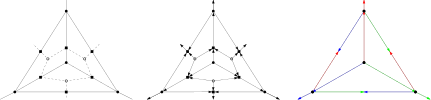
\includegraphics[width=0.95\textwidth]{alpha_ex.png}
  \caption{Der Primal-Duale Graph $K_4+K_4^*$ mit einer $\alpha_s$-Orientiertung und dem zugehörigen Schnyder Wood auf $K_4$. }
\end{figure}

\begin{theorem}\label{alpha_bij}
Sei $G$ ein planer Graph mit Aufhängungen $\{a_1,a_2,a_3\}$, dann sind die folgenden Strukturen in Bijektion:
\begin{itemize}
\item Die Schnyder Wälder auf $G$.
\item Die Schnyder Wälder auf dem (schwachen) dualen Graphen $G^*$.
\item Die $\alpha_{s}$-Orientierungen des Abschlusses von $G+G^*$ mit $\alpha_s(v) = \alpha_s(f) = 3$ für jeden Knoten-Knoten $v$ und Gebiets-Knoten $f$,  $\alpha_s(e) = 1$ für jeden Kanten-Knoten $e$ und  $\alpha_s(f_\infty) = 0$.
\end{itemize}
\end{theorem}
